\documentclass[12pt,letter]{article} 
\usepackage{graphicx} 
\usepackage[margin=1in]{geometry}
\usepackage{hyperref} 


\title{RFI Checker User's Guide} 
\author{Cosmin Deaconu} 


\begin{document} 
\maketitle 

\section{Introduction} 

\begin{figure} 
  \centering
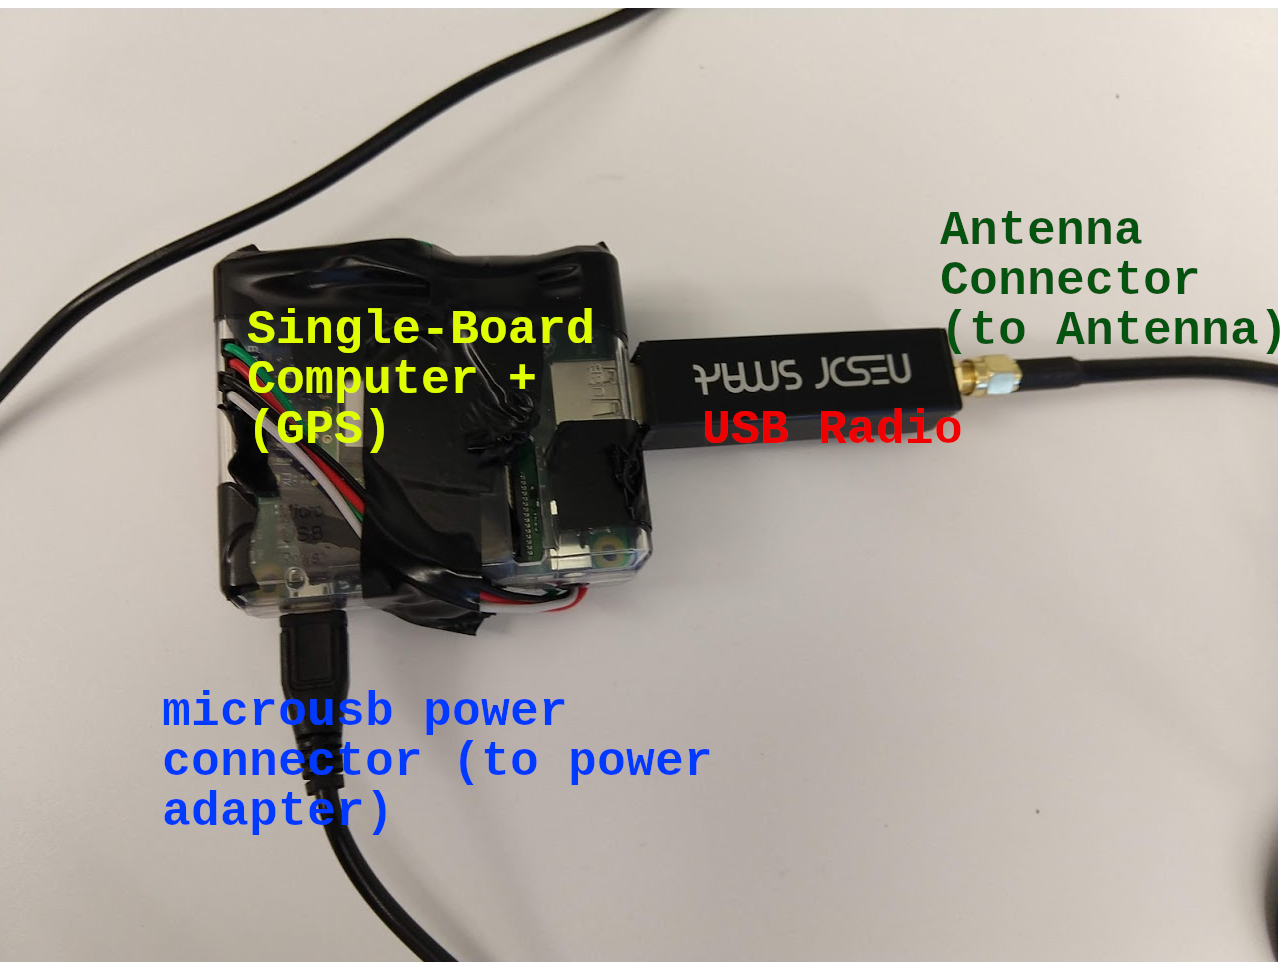
\includegraphics[width=5in]{overview} 
\caption{The RFI checker and its components} 
\end{figure}

RFI checker consists of a single-board computer (a Raspberry Pi 3A+)  with an
USB radio (RTL-SDR), an antenna plugging into the radio, a GPS, a microsd card (inside the RFI checker), and a power adapter (see Fig. 1).  
  
The RTL-SDR USB Radio  is a cheap USB device originally designed for digital TV
reception but turns out to be capable of acting as an inexpensive, configurable
radio. In this case, the Raspberry Pi is configured to start measuring the RF
spectrum on startup and dump data to the SD card. The data (time and position)
from the GPS (taped inside the case and connected via the jumper wires) is also
recorded while spectra are being taken, mostly to get a good time reference. 

The code running on the SBC (and this document) is available at \url{https://github.com/RNO-G/pi_rfi_checker} in case you are curious. 

\section{Assembly} 

The device was partially disassembled for shipping. To put back together: 
\begin{enumerate} 
\item Plug the USB Radio into the full-size USB port on the single-board computer
\item Plug the antenna into the USB radio (gold coaxial connector, hand tightening is fine). Note that it's possible that the antenna unscrewed itself from the base during shipping, so just make sure that's also secure. The antenna telescopes but the un-telescoped length is fine for the frequencies we are primarily interested in so no need to un-telescope. 
\item Plug the micro-usb part of USB to micro-usb cable (the one with the switch on it) into the SBC and the USB part into the power brick (don't plug the brick in until ready to take data!). 
\end{enumerate} 

\section{Usage} 

When powered, the Pi will boot and start taking spectra when it's done booting.
Note that the power cable has a toggle button on it.  Most likely it is in the
off state when unpacked (although it could have accidentally been pressed
during packing/shipping). So if you plug in the device and no LED's turn on,
then try the switch.

Booting takes about a minute and then each full spectrum takes around 40
seconds to capture.  Taking at least several spectra would be good so that we
can average them later. Each scan uses a bit less than a megabyte. Ideally you
wouldn't move the antenna too much while it's taking data, although it doesn't
matter so much. We are primarily interested in vertical polarization, so that
means that the antenna should roughly be pointing up. 

When you've taken at least a few scans, just turn it off with the off switch. 

\section{Retrieving Data} 

The micro-sd card is on the side opposite the full-size USB port that the radio
plugs into. If you push it in it should come out. Be careful, it is easy to
lose! A micro-SD to SD adapter was included with the checker. The data
partition on the SD card is formatted FAT-32 so it should be readable by any
computer. It might complain about a file system check when plugged in; this is
because we didn't turn off the computer cleanly, but the data should be fine. 

Each time it's turned on, data is placed in a new folder (labeled by run
number; the run number is incremented each time the device is powered on). The
first three (or maybe four) runs on the SD card were taken at Chicago before
sending it off.  The timestamps are probably wrong since the device is not
connected to the internet to update the time (and the GPS isn't used to set the
system time). 

\end{document} 

